\documentclass{article}
\usepackage[a4paper, total={6in, 9in}]{geometry}
\usepackage[utf8]{inputenc}
\usepackage[italian]{babel}
\usepackage[T1]{fontenc}
\usepackage{hyperref}
\usepackage{amsmath}
\usepackage{tikz}
\usepackage{natbib}
\usepackage{graphicx}
\usepackage{comment}
\usepackage{float}
\renewcommand{\baselinestretch}{1.5}

\usepackage[most]{tcolorbox}
\definecolor{block-gray}{gray}{0.9}
\newtcolorbox{Cit}{colback=block-gray,grow to right by=5mm,grow to left by=5mm,
boxrule=0pt,boxsep=0pt,breakable}

\usepackage{afterpage}

\newcommand\blankpage{%
    \null
    \thispagestyle{empty}%
    \addtocounter{page}{-1}%
    \newpage}

\graphicspath{ {./Immagini/} }

\begin{document}
\pagenumbering{gobble}

\afterpage{\blankpage}

\begin{titlepage}
   \begin{center}
   {\Large 
   \vspace*{1cm}

       \textbf{Elaborato Esame di Stato 2020/2021}

       \vspace{0.5cm}
        Analisi e progettazione della rete per un cinema multisala.
            
       \vspace{1.5cm}

       \textbf{Cornacchiari Roberto}\\
       \textbf{5A Informatica}\\
       \vspace{1cm}
        Docenti di riferimento:\\
        - Prof.ssa Foglio Laura\\
        - Prof. Pollini Andrea
       \vfill
       \vspace{0.8cm}
        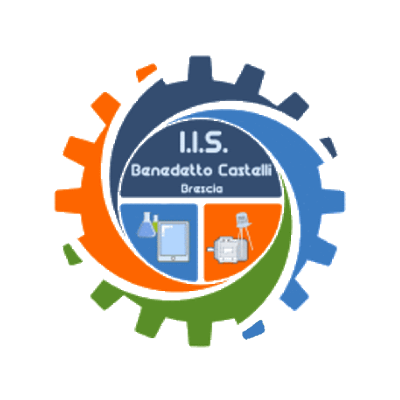
\includegraphics[width=5cm]{Logo.png}
        
       IIS Benedetto Castelli\\
       Brescia\\
       Italia\\
       Giugno 2021\\
       }
   \end{center}
\end{titlepage}

\afterpage{\blankpage}

\tableofcontents
\pagebreak

\pagenumbering{arabic}
\section{Introduzione}
L'analisi si sviluppa in più punti, andando a toccare i vari aspetti legati alla realizzazione della struttura hardware e software richiesta, usando competenze apprese nel corso degli anni nelle materie di indirizzo.

\subsection{Traccia}
\begin{quotation}
\textit{"Un cinema multisala deve riavviare la proiezione dei film dopo l'emergenza Coronavirus, rispettando le regole sull'affollamento e il distanziamento sociale. 
Si vuole dunque progettare un sistema che permetta agli addetti alle sale di registrare i dati degli spettatori man mano che entrano, in modo da poter ricostruire
eventuali contagi se successivamente qualcuno dovesse risultare positivo al COVID-19, rispettando comunque le tutele garantite dalla normativa sulla privacy.
Discutere come si potrebbe organizzare un tale servizio, sia da un punto di vista hardware che software, prendendo in considerazione le tematiche che si ritengono più rilevanti."}
\end{quotation}

\subsection{Sintesi soluzione proposta}
In questa sezione è presente un breve riassunto del sistema finale a cui sono giunto dopo l'analisi che ho svolto.

Il cinema presenta al suo interno più sale e ognuna di queste è dotata all'ingresso di una postazione (computer) da cui verranno erogati i biglietti e, all'interno, di una stanza di proiezione. Per poter accedere alla sala lo spettatore dovrà fornire un recapito telefonico che verrà verificato mediante un codice di 6 cifre inviato al numero dato. Questo permetterà alla gestione del cinema di risalire a tutti coloro che entreranno potenzialmente in contatto con un soggetto risultato positivo. I pc di queste postazioni fanno parte di una rete unica; all'interno di questa troviamo anche altri dispositivi (computer, stampanti e server NAS per il salvataggio dei film) situati nella sala amministrazione. Gli amministratori del cinema possono infatti aggiornare il catalogo dei film, aggiungere delle nuove rappresentazioni o risalire all'elenco  dei recapiti telefonici dei potenziali contagiati.

Per poter salvare questi dati viene utilizzato un database nel cloud al quale solo la rete sopracitata può accedere.

È inoltre presente una connessione Wi-fi per gli spettatori; questa viene collocata in una rete separata, in modo che non si possa accedere al sistema di gestione del cinema.


\section{Discussione della traccia}\label{sec:Ipotesi}

In questa sezione vengono approfonditi e decisi alcuni aspetti legati alla realtà proposta che permetteranno un'analisi tecnica più precisa.

\subsection{Privacy del cittadino}\label{sec:Privacy}

Per soddisfare quanto richiesto, dobbiamo fare in modo di tenere traccia degli accessi alle sale durante le proiezioni, avendo anche la possibilità, nel caso in cui uno spettatore risultasse positivo al Covid-19, di risalire a tutti coloro che fossero stati in contatto con lui.

Questo potrebbe essere facilmente fatto prendendo nota delle generalità di ogni persona che entra nella sala; i nominativi verrebbero poi forniti alle autorità competenti che provvederebbero a contattare gli interessati e a prescrivere loro un tampone.
Nascerebbe però un problema legato alla privacy, in quanto salvare informazioni personali (come nome e cognome o i dati del documento di identità) all'interno di database privati richiederebbe un notevole impegno burocratico, con il rischio di incorrere in sanzioni o denunce.

Onde evitare queste difficoltà burocratiche possiamo pensare di usare un altro sistema. Per il nostro scopo risulta adatto il recapito telefonico: registrando il numero di telefono, è possibile contattare in caso di necessità tutti coloro che sono entrati, senza salvare altri dati personali sensibili.

\subsection{Gruppi di persone}\label{sec:Gruppi}

Per quanto detto nella sezione \ref{sec:Privacy} ogni individuo che entra in una sala viene registrato con il numero di telefono che fornisce all'atto dell'acquisto del biglietto. Il caso ideale è quello in cui tutti gli spettatori si registrano con il proprio recapito telefonico. Questo potrebbe però non essere sempre possibile.

Uno spettatore potrebbe infatti non avere a disposizione un cellulare di cui fornire il numero, magari perché l'ha dimenticato o non l'ha portato con sé, oppure semplicemente perché si tratta di un bambino non ancora in possesso di uno smartphone venuto al cinema con i genitori.

Per permettere anche a costoro l'accesso alle sale possiamo decidere che, nel momento del rilascio del biglietto, su di esso venga scritto da quante persone è composto quel gruppo (questo risulta anche utile per gestire lo spazio in sala). Sarà poi compito dell'intestatario del numero indicato informare il cinema qualora uno dei membri del gruppo dovesse risultare positivo al Covid-19.

\subsection{Verifica del recapito}\label{sec:Sicurezza}

Nella sezione \ref{sec:Privacy} abbiamo stabilito di utilizzare il recapito telefonico per tenere traccia delle presenze. Dobbiamo però accertarci che lo spettatore non fornisca un numero di telefono fasullo o che semplicemente sbagli a dettarlo all'operatore.

Per evitare questa situazione, dopo aver comprato il biglietto e quindi fornito il numero, prima dell'ingresso in sala, allo spettatore verrà chiesto di leggere il codice di 6 cifre inviato tramite SMS, così da verificare la correttezza del recapito. Una volta confermato anche questo codice il singolo spettatore o il gruppo potrà prendere posto (il funzionamento di questo servizio viene approfondito nella Sezione \ref{sec:Messaggistica}).

\subsection{Accesso e sicurezza}\label{sec:Login}

Bisogna evitare che utenti non autorizzati possano agire sul database; questo vuol dire impedire agli spettatori o in generale ai non addetti di utilizzare i software applicativi che dialogano con la base di dati. Il modo migliore di fare questo è impostare che per accedere alle macchine vengano richieste delle credenziali note soltanto agli operatori (ossia richiedere la password in fase di accensione, come avviene normalmente in tutti i dispositivi, qualsiasi sia il sistema operativo installato).

Un'altra soluzione sarebbe quella di predisporre un login all'interno dell'applicazione, ma effettuando l'accesso nella fase iniziale si garantirebbe una maggiore sicurezza del sistema. Un computer infatti, anche senza gli applicativi che comunicano con il database, consente l'accesso al server NAS e quindi ai film (vedi sezione \ref{sec:NAS}).

\section{Infrastruttura di rete}\label{sec:Infrastruttura}

In questa sezione vengono presi in esame gli aspetti legati all'infrastruttura hardware da realizzare per soddisfare le necessità del sistema.

\subsection{Sportelli di ingresso}\label{sec:Sportelli}

All'ingresso delle sale è necessario poter controllare, tramite il codice inviato via SMS, la correttezza del recapito fornito. Si può quindi pensare di delegare a queste postazioni di controllo anche la funzione di biglietteria: uno spettatore cerca in che sala viene proiettata la pellicola che gli interessa e vi si reca. Qui si mette in fila (rispettando il distanziamento previsto dalle norme anti-covid) per prendere il biglietto. Quando è il suo turno dichiara da quante persone è formato il gruppo (vedi Sezione \ref{sec:Gruppi}) e detta il numero di telefono all'operatore, in quale gli chiederà il codice di conferma inviato tramite SMS. Se il codice corrisponde a quello visualizzato sullo schermo dell'addetto alla biglietteria, lo spettatore (o il gruppo) viene registrato nel sistema e accede alla sala.

Utilizzando questo sistema possiamo inserire una postazione al posto di due (biglietteria e controllo all'ingresso), risparmiando in termini di dispositivi e di cablaggio.

Tutte le macchine sono collegate allo stesso switch e fanno parte della stessa rete.

\subsection{Stanza di proiezione}\label{sec:Proiettori}

Ogni sala del cinema deve disporre di una piccola stanza, opposta rispetto allo schermo, dove situare il proiettore e il computer su cui far vedere il film (le pellicole ormai sono state sostituite da file multimediali). Serve dunque collegare alla rete anche questi terminali, così che possano accedere allo spazio di archiviazione dei film da cui li scaricano (vedi Sezione \ref{sec:NAS}).

\subsection{Sala amministrazione}\label{sec:Amministrazione}

All'interno del cinema è necessaria una sala amministrazione, accessibile solo al personale autorizzato. Qui vanno installati dei pc per poter gestire i dati del database.
Questi computer sono connessi, come quelli indicati nelle sezioni precedenti, alla stessa rete via cavo. Questa Lan, e solo questa, ha accesso al server database (vedi Sezione \ref{sec:MySQL}).

Oltre a questi dispositivi sono presenti anche delle stampanti a supporto della parte burocratica.

\subsection{Server utilizzati}\label{sec:Database}

\subsubsection{Database MySQL}\label{sec:MySQL}
In questo paragrafo vengono approfondite e discusse le possibili scelte per quanto riguarda il database.
Dato che non sono presenti interazioni tra spettatori e base di dati, le macchine che possono accedervi sono sempre le stesse, ossia quelle degli sportelli e della sala amministrazione. Possiamo quindi dire che il server deve essere accessibile unicamente dalla Lan che comprende tutte queste macchine e che i loro indirizzi ip e MAC address saranno sempre gli stessi (questo facilita la scrittura di eventuali ACL).
\begin{quote}
\begin{Cit}
\textit{
Una \textbf{ACL (Access control list)}, è un insieme di regole usato per esprimere e/o definire l'accesso o meno ad alcune risorse di un sistema informatico da parte degli utenti.\\
La singola regola di una ACL si chiama \textbf{ACE (Access control entry)}, la quale può essere di consenso o di negazione.\\
Le ACL possono essere: standard se viene indicata solo la sorgente del traffico (identificate da un numero compreso tra 1 e 99), estese se invece viene specificata anche la destinazione del messaggio (numeri da 100 a 199).}
\end{Cit}
\end{quote}

Esistono due diverse possibilità da considerare:
\begin{itemize}
    \item \textbf{Server proprietario: }prevede che il server usato come database sia acquistato e completamente gestito dalla società (in questo caso il cinema); i vantaggi di questa soluzione sono la possibilità di organizzare come si vuole ogni aspetto, hardware o software, ma obbliga anche alla gestione della sicurezza e dell'integrità dei dati. Tutto questo si traduce in ingenti costi di messa in opera e di manutenzione continua. Uno schema logico di come sarebbe la rete adottando questa proposta è rappresentato nell'immagine \ref{fig:SchemaDatabaseInterno}.
    \begin{figure}[H]
    \centering
    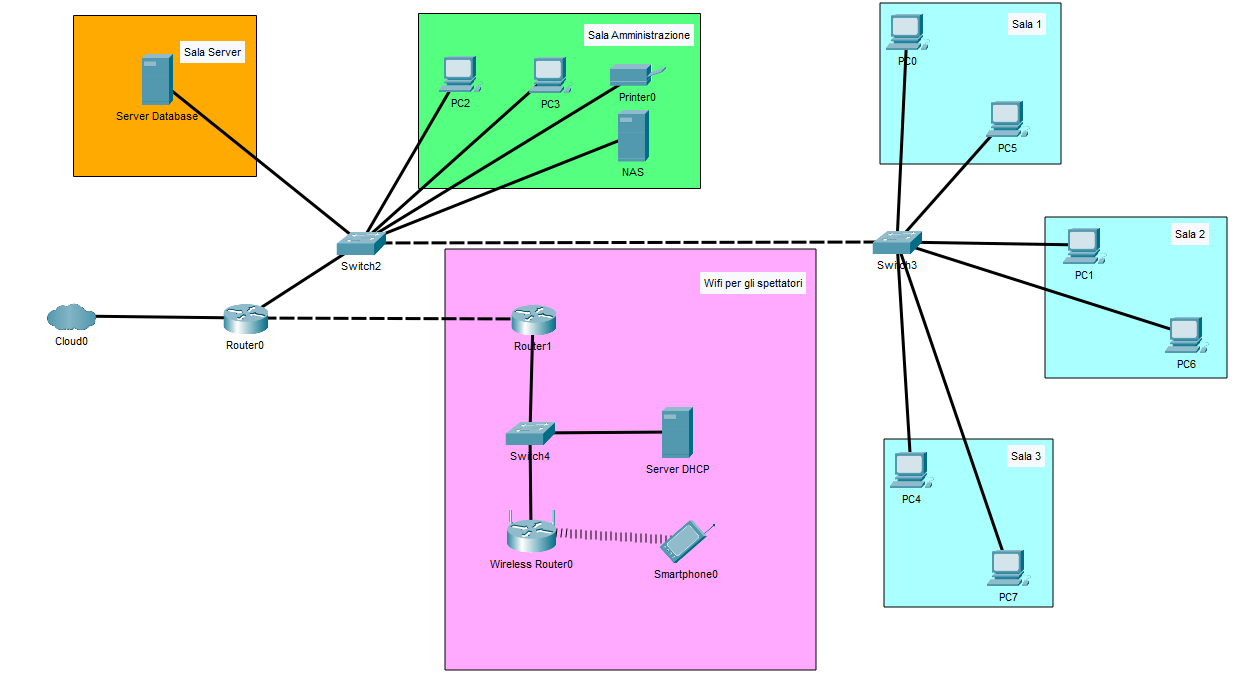
\includegraphics[width=14cm]{SchemaReteDatabaseInterno.png}
    \caption{Schema della rete con server proprietario}
    \label{fig:SchemaDatabaseInterno}
    \end{figure}
    \item \textbf{Server nel cloud: }la società, invece di acquistare fisicamente i server, dovendo quindi predisporre gli spazi e il servizio di manutenzione e di sicurezza, può decidere di affittare il servizio di cui ha bisogno (in questo caso di un database dove salvare i dati di film, proiezioni e spettatori), delegando quindi le responsabilità e abbassando i costi.
    
    Questa soluzione è sicuramente preferibile: si ha una notevole riduzione dei costi e la gestione viene affidata a dei fornitori specializzati. Si genera quindi un servizio IaaS a canone variabile: maggiore sarà il numero di richieste e l'utilizzo, maggiori saranno i costi.
    
    \begin{quote}
    \begin{Cit}
    \textit{
    \textbf{IaaS (Infrastructure as a Service)} is a form of cloud computing that provides virtualized computing resources over the internet.
    In the IaaS model, the cloud provider manages IT infrastractures such as storage, server and networking resources, and delivers them to subscriber organizations via virtual machines accessible through the internet.}
    \end{Cit}
    \end{quote}
    
    Utilizzando un server remoto, lo schema della rete (che rappresenta quindi lo schema effettivamente implementato all'interno della realtà proposta) è visibile nell'immagine \ref{fig:SchemaDatabaseEsterno}.
    
    \begin{figure}[H]
    \centering
    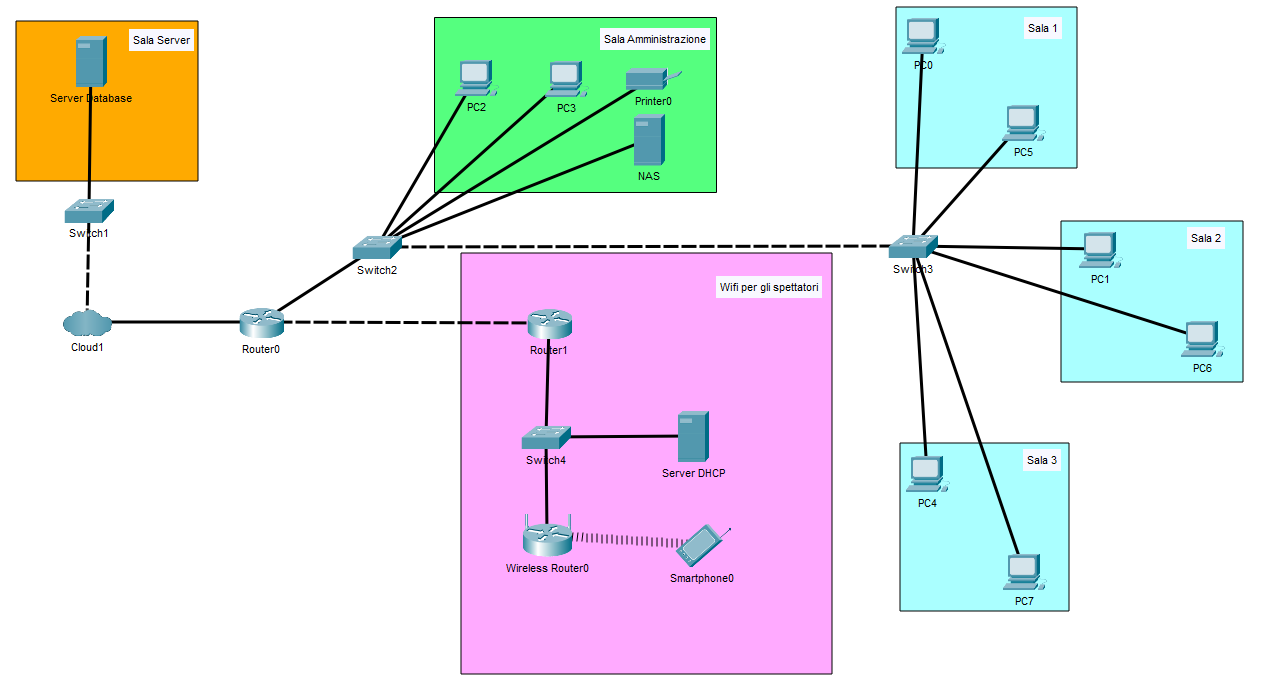
\includegraphics[width=\textwidth]{SchemaReteDatabaseEsterno.png}
    \caption{Schema effettivo della rete (server nel cloud)}
    \label{fig:SchemaDatabaseEsterno}
    \end{figure}
    \end{itemize}

\subsubsection{Server NAS}\label{sec:NAS}
Al fine di archiviare i film e per renderli disponibili a tutti i pc delle sale proiezione, viene installato un server NAS all'interno della rete.

\begin{quote}
    \begin{Cit}
    \textit{
    Un \textbf{NAS (Network Attached Storage)} è un dispositivo collegato alla rete che permette di condividere con tutti gli utenti dello spazio di archiviazione comune; su di esso è possibile caricare e modificare file visibili da tutti i device connessi (è  come se si avessero più dischi rigidi all'interno del proprio computer).}
    \end{Cit}
    \end{quote}

Installiamo quindi un server di questo tipo all'interno della sala amministrazione (un NAS occupa solitamente lo spazio di un pc fisso) e lo colleghiamo alla rete. Sarà poi compito dell'operatore in sala proiezione accedervi e trasferire sul computer il film da trasmettere.

\section{Indirizzi IP e controllo del traffico}\label{sec:IPeACL}

Dopo aver definito lo schema logico dei dispositivi di cui è composta la rete (vedi Figura \ref{fig:SchemaDatabaseEsterno}) bisogna distribuire gli indirizzi di essi e impostare le opportune ACL per limitare il traffico.

\subsection{Assegnazione indirizzi IP}\label{sec:IndirizziIp}

Per quanto riguarda la \textbf{LAN} del cinema, vengono assegnati degli indirizzi statici appartenenti alla rete \textbf{200.200.200.0/24} a tutte le macchine. Sono statici in quanto non sono previsti continui cambiamenti dei dispositivi che ne fanno parte; può succedere che vengano installati nuovi computer, ma in questo caso basta fornire loro un indirizzo libero.

Il \textbf{wi-fi} per gli ospiti è gestito da un wireless router posizionato al centro del cinema (o nel punto da cui si copre la maggior parte della struttura). Questo router distribuisce dinamicamente tramite il server DHCP gli indirizzi della rete \textbf{120.10.0.0/22} (la classe C fornisce al massimo $2^{8}-2$ host, non sufficienti per le esigenze di un cinema; si può quindi preferire una classe C a cui applicare un supernetting, in modo da aumentare gli host a disposizione $2^{10}-2$ indirizzi risulta più appropriata).

Il servizio wi-fi viene fornito mediante protocollo WPA2 Personal. Per collegarsi è quindi necessario utilizzare la password che viene indicata in alcuni volantini sparsi per la struttura.

\begin{quote}
    \begin{Cit}
    \textit{
    Un \textbf{server DHCP(Dynamic Host Configuration Protocol)} ha il compito di assegnare ad un dispositivo che si connette alla sua rete il primo indirizzo ip disponibile e la configurazione necessaria per navigare nella rete stessa (indirizzo di gateway, DNS...).}
    \end{Cit}
    \end{quote}
    
Il provider del cloud, all'atto dell'acquisto, fornisce l'indirizzo statico da usare per collegarsi al \textbf{database}. Per ipotesi questo indirizzo è \textbf{79.72.250.7/8}.

\subsection{Definizione delle ACL}

Per garantire la sicurezza bisogna impostare sulle interfacce dei router alcune ACL.

In particolare vogliamo che:
\begin{itemize}
    \item soltanto la LAN del cinema possa accedere al database sul cloud;
    \item gli spettatori non possano accedere alla LAN;
    \item nelle 2 reti possa entrare solo del traffico "di ritorno", ossia delle risposte a delle richieste o connessioni precedentemente fatte dall'interno.
\end{itemize} 
È possibile raggiungere questi obiettivi con 2 ACL estese (in quanto va indicata anche la destinazione) opportunamente scritte.

La prima viene inserita nell'interfaccia del Router0 che porta alla rete wi-fi (rosa nell'immagine) in ingresso (viene quindi verificato il traffico che entra nel router da quella porta).
\begin{verbatim}
    deny tcp 120.10.0.0 0.0.255.255 host 79.72.250.7 eq 80
    deny tcp 120.10.0.0 0.0.255.255 host 79.72.250.7 eq 20
    deny tcp 120.10.0.0 0.0.255.255 host 79.72.250.7 eq 21
    deny ip 120.10.0.0 0.0.255.255 200.200.200.0 0.0.0.255
    permit ip 120.10.0.0 0.0.255.255 any
\end{verbatim}
Le prime 3 righe negano l'accesso tramite http e ftp al database, la quarta blocca qualsiasi tipo di comunicazione con il cinema e l'ultima permette tutto il rimanente traffico verso internet.

L'altra ACL va invece posizionata all'ingresso proveniente da internet nel Router0.
\begin{verbatim}
    permit tcp any any established
    deny ip any any
\end{verbatim}
La prima riga consente l'accesso solo a connessioni tcp già instaurate, mentre la seconda impedisce tutto il resto.

\subsection{Camuffamento degli indirizzi tramite NAT}

\begin{quote}
    \begin{Cit}
    \textit{
    Il \textbf{NAT (Network address translation)} è un processo attivo su un apparato di rete (router, firewall, ...) che ha il compito di modificare l'indirizzo ip dei messaggi che transitano da un'interfaccia ad un'altra. Viene usato per mascherare gli indirizzi ip privati degli host, usando invece indirizzi pubblici.}
    \end{Cit}
    \end{quote}
    
Per garantire una maggior sicurezza al sistema, si può impostare sul router di frontiera (ossia quello situato all'uscita della rete verso internet) un processo di NAT, in modo da nascondere gli indirizzi privati delle macchine.

\section{Servizio di messaggistica}\label{sec:Messaggistica}
Nella Sezione \ref{sec:Sicurezza} si è deciso di richiedere allo spettatore il recapito telefonico e di inviargli un codice di conferma.

Per poter effettuare questa procedura in maniera automatizzata bisogna integrare il messaggio all'interno del software applicativo degli sportelli. Sul web sono disponibili vari servizi che consentono di fare questo al prezzo di pochi centesimi al messaggio (circa 0,04€ ogni SMS inviato). Dato che ormai quasi tutta la popolazione possiede uno smartphone con installata un'app di messaggistica (whatsapp, telegram, ...), si possono anche usare direttamente l'API messe a disposizione da queste app che consentono di inviare messaggi direttamente dal software (sempre ad un prezzo molto basso).

\begin{quote}
    \begin{Cit}
    \textit{
    Un' \textbf{API (Application Programming Interface)} consente agli sviluppatori esterni di accedere a determinate funzionalità di un altro programma. Sono un modo con il quale i programmatori espongono all'esterno delle funzionalità del proprio prodotto. Sono spesso usate per realizzare ed integrare tra loro software applicativi.}
    \end{Cit}
    \end{quote}

\section{Diagramma entità relazione}\label{sec:ER}

Questa sezione è dedicata all'analisi dello schema relazionale che andrà implementato nel database.

\begin{quote}
\begin{Cit}
\textit{
Il \textbf{diagramma E-R} è un modello concettuale usato per rappresentare logicamente scenari reali e come le entità si relazionano tra di loro. Viene spesso utilizzato nella prima fase della progettazione di un database in quanto rende veloce la realizzazione delle tabelle e chiare le chiavi (primarie o esterne) che dovranno essere utilizzate.}
\end{Cit}
\end{quote}

\begin{figure}[h]
    \centering
    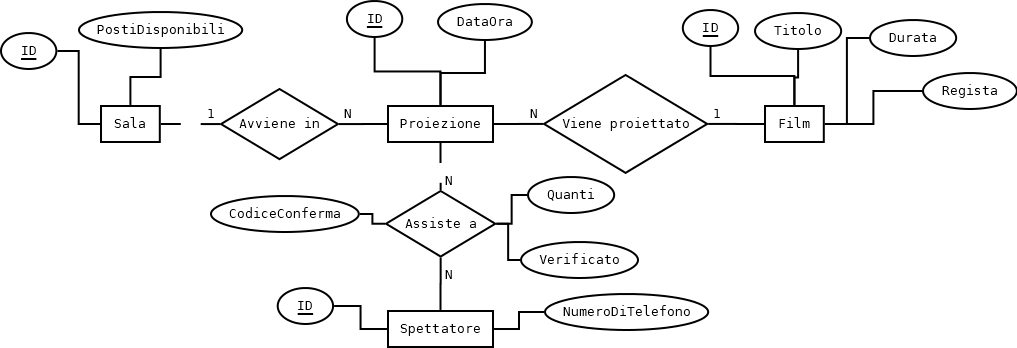
\includegraphics[width=\textwidth]{ERElaborato.png}
    \caption{Diagramma entità relazioni}
    \label{fig:ER}
\end{figure}

Come possiamo vedere dalla figura \ref{fig:ER}, il nostro modello presenta 4 entità (i rettangoli) che rappresentano: 
\begin{itemize}
    \item \textbf{sala: }una delle sale presenti nella struttura, con relativa capienza massima;
    \item \textbf{film: }un singolo film presente nel catalogo del cinema con relative informazioni;
    \item \textbf{proiezione: }una singola riproduzione programmata di un film in una sala;
    \item \textbf{spettatore: }il singolo spettatore (o gruppo, nel caso in cui una persona non fosse provvista di cellulare) che partecipa a una rappresentazione;
\end{itemize}
Ogni entità, oltre agli attributi di facile comprensione, presenta un ID, ossia un identificatore unico della singola, che verrà utilizzato come chiave primaria all'interno di ogni tabella del database.
\begin{quote}
\begin{Cit}
\textit{
Una \textbf{chiave primaria}, nel modello relazionale delle basi di dati, è un insieme di attributi che permette di individuare univocamente una riga (o record) in una tabella o relazione.}
\end{Cit}
\end{quote}

Queste entità sono legate da 3 relazioni (rombi) che indicano:
\begin{itemize}
    \item \textbf{avviene in: }una proiezione avviene in una e una sola sala, ma in una sala possono verificarsi nessuna o tante riproduzioni;
    \item \textbf{viene proiettato: }un film può essere rappresentato più volte, ma durante una proiezione si può assistere solo ad una pellicola;
    \item \textbf{assiste a: }una persona registrata nel database può andare al cinema più volte e ad ogni proiezione partecipano un certo numero di persone (minimo 0, massimo la capienza della sala).
\end{itemize}

Quest'ultima relazione è diversa dalle altre; essendo una N a N può infatti presentare attributi (in quanto nella successiva realizzazione del database diventerà una tabella assestante). Il perché di questi attributi è stato descritto nelle Sezioni \ref{sec:Gruppi} e \ref{sec:Sicurezza} a pagina \pageref{sec:Gruppi}.


\section{Sviluppo software}\label{sec:SviluppoSoftware}
In questa sezione vengono indicati i vari aspetti e le decisioni che sono state prese in merito alla realizzazione del software di gestione.

\subsection{Configurazione database}\label{sec:ConfigurazioneDatabase}
Nella Sezione \ref{sec:ER} è stato mostrato il diagramma E-R che rappresenta la realtà proposta. Questo schema deve essere convertito in tabelle all'interno del database presente sul cloud. 
Si usano i comandi DDL per la creazione dello schema e delle tabelle, impostando anche tutti i vincoli di integrità referenziale indicati dalle relazioni.

\begin{quote}
    \begin{Cit}
    \textit{
    Il \textbf{DDL (Data Definition Language)} è un linguaggio per la definizione della struttura dei dati; è usato principalmente dall'amministratore del sistema ed è costituito da comandi che consentono di definire e modificare la struttura della base di dati e dei vincoli di integrità.}
    \end{Cit}
    \end{quote}
    
Lo schema che si viene così a creare è mostrato in Figura \ref{fig:SchemaTabelleDatabase}. Le frecce blu che collegano tra di loro le tabelle sono i vincoli di integrità referenziale.

\begin{quote}
    \begin{Cit}
    \textit{
    Un \textbf{vincolo di integrità referenziale} è un vincolo di tipo interrelazionale, ovvero una proprietà dei dati la quale, per essere soddisfatta, richiede che ogni valore di un attributo (colonna) di una relazione (tabella) esista come valore di un altro attributo in un'altra relazione.}
    \end{Cit}
    \end{quote}
    
    \begin{figure}[H]
    \centering
    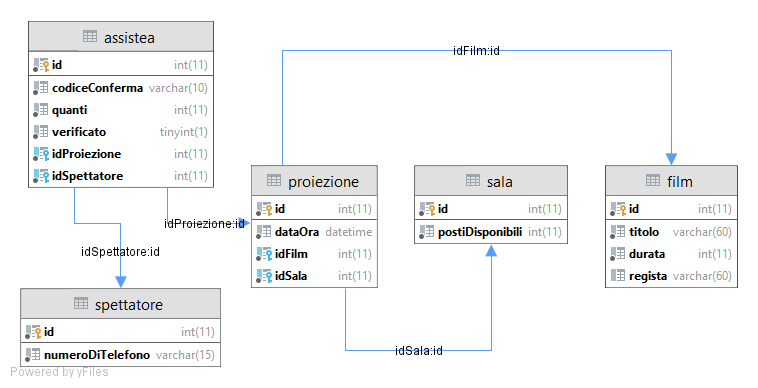
\includegraphics[width=\textwidth]{SchemaDatabase.png}
    \caption{Schema relazionale database}
    \label{fig:SchemaTabelleDatabase}
    \end{figure}

\subsection{Software applicativi}\label{sec:Applicativo}
Per permettere al personale di accedere ai dati si devono realizzare dei programmi da installare sui pc previsti.

La scelta migliore è quella di sviluppare 2 applicazioni desktop da installare sui computer: 
\begin{itemize}
    \item la prima, presente nei pc all'ingresso delle sale, permette all'operatore di registrare un nuovo accesso, inserendo il numero di telefono e le persone di cui è composto il gruppo; dopo aver inserito questi valori viene inviato al recapito fornito il messaggio contenente il codice a 6 cifre che l'utente detta all'addetto. Se il codice è corretto viene registrato l'accesso alla sala nel database e gli spettatori si possono accomodare.
    \item la seconda, da installare sulle macchine della sala amministrazione, permette di aggiungere nuovi film al catalogo, di programmare nuove proiezioni e di risalire all'elenco dei recapiti telefonici degli spettatori presenti in una sala durante una riproduzione.
\end{itemize}

Questi programmi sono abbastanza semplici e leggeri e non necessitano di hardware potenti per essere eseguiti (ciò porta anche ad un risparmio nell'acquisto delle macchine da posizionare nel cinema). Non vi è quindi nessun vincolo particolare per la scelta del linguaggio o dei linguaggi da utilizzare per il loro sviluppo. Dovendo gestire la comunicazione con il database e dovendo interpretare i dati che questo invierà, si può pensare di utilizzare \textbf{JavaScript}, in quanto gestisce in maniera quasi immediata file in formato JSON; è inoltre estremamente versatile e possiede numerose librerie e framework che ampliano notevolmente le possibilità di sviluppo.

JavaScript nativamente è utilizzato per realizzare siti web dinamici e infatti viene eseguito all'interno del browser. Per realizzare applicazioni desktop bisogna quindi utilizzare uno dei tanti framework disponibili: ad esempio \textbf{Electron}. Il suo scopo è quello di consentire la creazione di GUI (Graphical User Interface) di applicazioni utilizzando tecnologie web (con Electron sono stati sviluppati grandi ed estremamente diffusi software come Visual Studio Code, Microsoft Teams, Discord, Slack e molti altri).

\subsection{Interazione con la base di dati}\label{sec:InterazioneBaseDati}
Per poter interagire con il database vengono utilizzati dei piccoli programmi (script) scritti in linguaggio PHP; questi presentano al loro interno una connessione al server e riescono a eseguire determinate operazioni.
Bisogna quindi prevedere uno script per ogni funzionalità da implementare nell'applicativo che deve avere accesso ai dati.

Queste operazioni possono essere di lettura, quando l'app vuole mostrare delle informazioni (ad esempio la lista degli spettatori in una data proiezione), o di scrittura, quando bisogna inserire nuovi dati (spettatori, film...). Per fare questo si usano i comandi DML.

\begin{quote}
    \begin{Cit}
    \textit{
    Il \textbf{DML (Data Manipulation Language)} è un linguaggio che consente di leggere, inserire, modificare o eliminare i dati in un database.}
    \end{Cit}
    \end{quote}
    
Questi script vengono poi chiamati dagli applicativi installati sui computer del cinema. La comunicazione tra questi 2 software avviene mediante il meccanismo delle fetch API. All'interno del codice front-end è quindi possibile invocare l'opportuno script, il quale viene eseguito, agisce sul database e ritorna una risposta contenente i dati richiesti in formato JSON o una conferma dell'avvenuta operazione.

\begin{quote}
    \begin{Cit}
    \textit{
    La \textbf{fetch API} è un'interfaccia che consente di effettuare richieste HTTP ad un server da un browser web utilizzando l'url della risorsa (nel nostro caso dello script) che si vuole recuperare.}
    \end{Cit}
    \end{quote}

\end{document}
